
Shared libraries are basically object files, that are loaded, (if not already) at runtime
when a process linked against it starts execution. The pages remain in the memory until
they are swapped out by pages from another program, based upon the page replacement algorithms\cite{pageReplacement}.

Shared libraries are useful because of multiple reasons. They allow programmers to make use of existing
code without increasing the executable sizes. Additionally, as there is a single copy of shared code, there
are fewer page faults because its possible that some other process may have already loaded the shared code.
In addition to this, shared libraries also make it easy to upgrade to newer versions of the code.

\begin{figure}
    \centering
    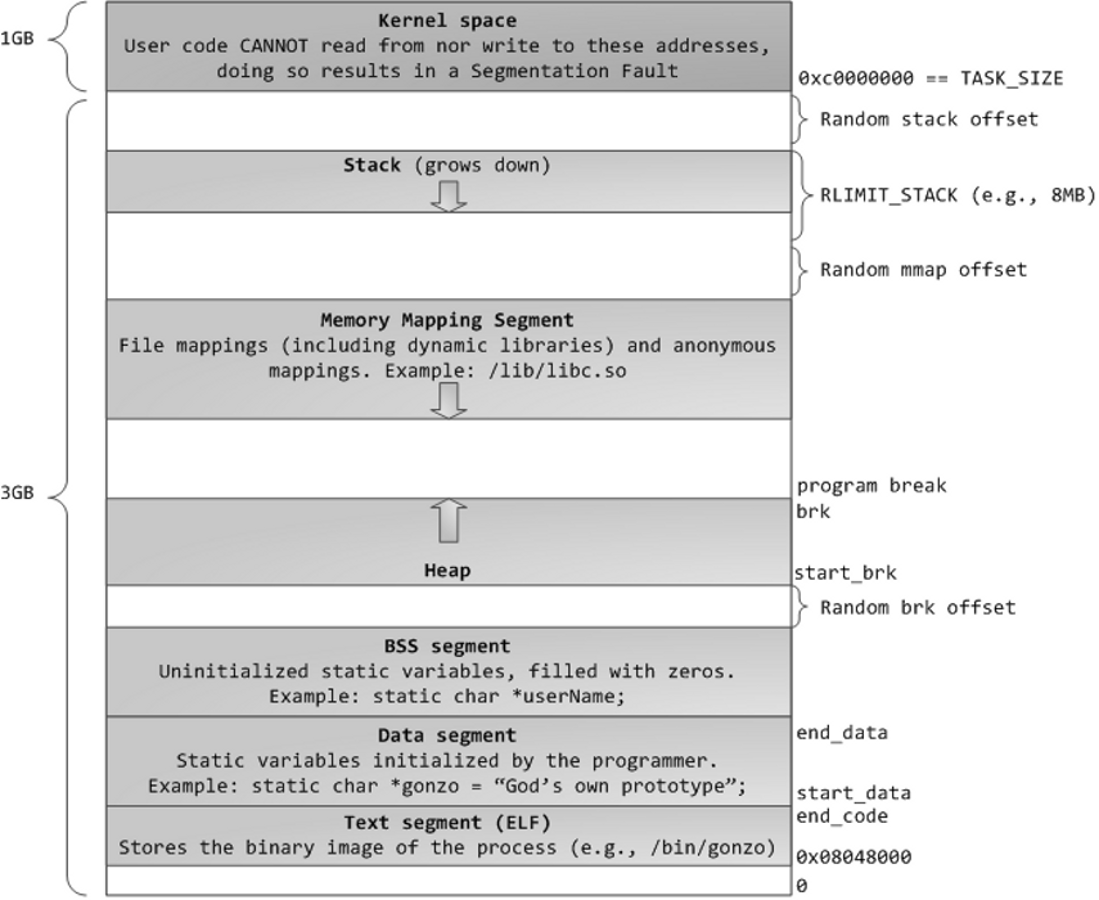
\includegraphics[width=\linewidth, height=8.5cm]{linuxFlexibleAddressSpaceLayout.png}
    \caption{Anatomy of a program in memory, Image Source:\cite{anatomyOfProgramInMemory}}
    \label{fig:processInMemory}
\end{figure}

Figure \ref{fig:processInMemory} shows how a running program looks like in the memory. Shared libraries, can be
loaded elsewhere in the memory, and the address mappings are stored in the memory mapping segment.
Size of a shared library depends upon the text-section, (which is mostly the shared-code and read-only data) and
the data and bss sections, which correspond to global and uninitialized data respectively. Figure \ref{fig:sizeOutput}
shows the result of \textit{size} command on the libnuma shared library. It can also be seen that, most of the shared
libraries on a normal linux-like systems are small, that is, less than 2 MBs. As such, they can easily fit in the
processor caches, and performance impact due to NUMA overhead would be negligible. However, some shared libraries
are big, (figure \ref{fig:libSizes} lists some big libraries) and we may have even bigger libraries in future.
Therefore, it is worthwhile to evaluate the performance impact in context of NUMA machines and perform possible
optimizations.

\begin{figure}
    \centering
    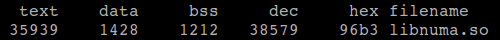
\includegraphics[width=\linewidth]{sizeOutput.png}
    \caption{output of \textit{size} command on libnuma.so}
    \label{fig:sizeOutput}
\end{figure}

\begin{figure}
    \centering
    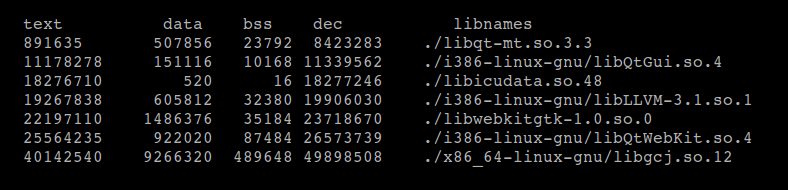
\includegraphics[width=\linewidth, height=2.5cm]{libSizes.png}
    \caption{Sizes for some big libraries}
    \label{fig:libSizes}
\end{figure}
